Dans tout ce chapitre, on considère \({(X_n)}_{n\geq 1}\) 
une suite de variables aléatoires réelles (ou complexes)
définies sur un espace probabilisé \((\Omega, \scr F, \bb P)\)
et une variable aléatoire \(X\) réelle (ou complexe).

\section{Différents modes de convergence} % 3.1

\subsection{Convergences presque sûre et probabilité} % 3.1.1

\begin{definition}
    On dit que \(X_n\) converge \defemph{presque sûrement} vers
    \(X\) et on note \(X_n \cvpsn X\),
    si
    \begin{equation*}
        \bb P(X_n \underset{n\to\infty}{\longrightarrow} X)
        = \bb P\left(\left\{\omega \in \Omega \mid X_n(\omega) \underset{n\to\infty}{\longrightarrow} X(\omega)\right\}\right)
        = 1.
    \end{equation*}
\end{definition}

\begin{remark}\,
    \begin{enumerate}
        \item Cela correspond à la convergence presque partout pour la
        mesure de probabilité \(\bb P\).

        \item Si \(X_n \cvpsn X\)
        et si \(h: \R \to \R\) est une fonction continue, alors
        \(h(X_n) \cvpsn h(X)\). En particulier, si
        \(X_n \cvpsn X\) et \(Y_n \cvpsn Y\), alors
        \begin{equation*}
            aX_n + bY_n \cvpsn aX + bY,\quad a, b \in \R.
        \end{equation*}
        et
        \begin{equation*}
            X_n Y_n \cvpsn XY.
        \end{equation*}
    \end{enumerate}
\end{remark}

\begin{definition}
    On dit que \({(X_n)}_{n\geq 1}\) converge \defemph{en probabilité} vers
    \(X\) si
    \begin{equation*}
        \forall \varepsilon > 0,\bb P(\n{X_n - X} \geq \varepsilon) \underset{n\to\infty}{\longrightarrow} 0.
    \end{equation*}
    On note alors \(X_n \cvp X\).

    Cela signifie que la probabilité que \(X_n\) s'écarte de \(X\)
    d'un écart supérieur à \(\varepsilon\) tend vers 0 lorsque
    \(n\) tend vers l'infini.
\end{definition}

\begin{example}
    \ptr{} On considère \(X_n\sim \mathcal E(n)\)
    % insert a graph here of the exponential distribution for n = 1, 2, 3, 4
    % representation de densites f_n de X pour n = 1...4, f_n(x) = n e^{-nx}
    \begin{center}
        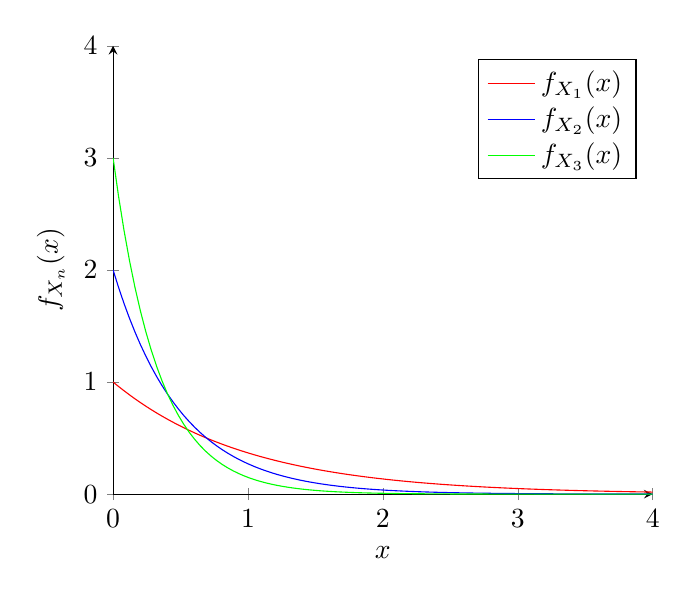
\begin{tikzpicture}
            \begin{axis}[
                axis lines = left,
                xlabel = \(x\),
                ylabel = {\(f_{X_n}(x)\)},
                xmin = 0,
                xmax = 4,
                ymin = 0,
                ymax = 4,
                legend pos = north east,
            ]
            \addplot [
                domain=0:4,
                samples=100,
                color=red,
            ]
            {exp(-x)};
            \addlegendentry{\(f_{X_1}(x)\)}
            \addplot [
                domain=0:4,
                samples=100,
                color=blue,
            ]
            {2*exp(-2*x)};
            \addlegendentry{\(f_{X_2}(x)\)}
            \addplot [
                domain=0:4,
                samples=100,
                color=green,
            ]
            {3*exp(-3*x)};
            \addlegendentry{\(f_{X_3}(x)\)}
            \end{axis}
        \end{tikzpicture}
    \end{center}
    Regardons \(\bb P(\n{X_n} \geq \varepsilon)\):
    \begin{equation*}
        \begin{aligned}
            \bb P(\n{X_n} \geq \varepsilon)
            &= \bb P(X_n \geq \varepsilon)\\
            &= \int_\varepsilon^{+\infty} n e^{-nx} \der x\\
            &= \ff{-e^{-nx}}_\varepsilon^{+\infty}\\
            &= e^{-n\varepsilon}.
        \end{aligned}
    \end{equation*}
    Donc \(X_n \cvpn 0\).

    On peut montrer que \(X_n \cvpsn 0\) (en TD).
\end{example}

\begin{proposition}
    Si \(X_n \cvpsn X\), alors \(X_n \cvp X\).
\end{proposition}

\begin{proof}
    Soit \(\varepsilon > 0\). On a
    \begin{equation*}
            \bb P(\n{X_n - X} \geq \varepsilon)
            = \bb E[\color{red}\underbrace{\color{black}\one_{\n{X_n - X} \geq \varepsilon}}_{f_n\underset{n\to\infty}{\to}0-\text{p.p.}}\color{black}]
    \end{equation*}
    Comme \(\n{f_n}\leq 1\) qui est intégrable, le théorème de convergence
    dominée donne
    \begin{equation*}
        \bb P(\n{X_n - X} \geq \varepsilon)
        = \bb E[\lim_{n\to\infty} \one_{\n{X_n - X} \geq \varepsilon}]
        = 0.
    \end{equation*}
\end{proof}

\begin{example}[Réciproque fausse]
    On considère \({(X_n)}_{n\geq 1}\) une suite de variables aléatoires
    de loi
    \begin{equation*}
        \bb P(X_n = n) = \frac{1}{n},\quad\text{et}\quad \bb P(X_n = 0) = 1 - \frac{1}{n}.
    \end{equation*}
    Soit \(\varepsilon >0\). Alors
    \begin{equation*}
        \bb P(\n{X_n} \geq \varepsilon)
        \leq \frac1n \underset{n\to\infty}{\longrightarrow} 0.
    \end{equation*}
    donc \(X_n \cvpn 0\).

    Supposons que les \({(X_n)}_{n\geq 1}\) sont indépendantes.
    Les événements \(A_n = \{X_n = n\}\) sont indépendants
    et vérifient
    \begin{equation*}
        \begin{aligned}
            \sum_{n=1}^{+\infty} \bb P(A_n) 
            &= \sum_{n=1}^{+\infty} \bb P(X_n = n)\\
            &= \sum_{n=1}^{+\infty} \frac{1}{n}\\
            &= +\infty.
        \end{aligned}
    \end{equation*}
    Donc par Borel-Cantelli, on a
    \begin{equation*}
        \bb P(\limsup_{n\to\infty} A_n) = 1.
    \end{equation*}
    Donc avec probabilité 1, \(X_n\) prend la valeur \(n\) 
    une infinité de fois. Donc avec probabilité 1, 
    \({(X_n)}_{n\geq 1}\) ne converge pas vers 0.
    Donc \({(X_n)}_{n\geq 1}\) ne converge pas presque sûrement.
\end{example}

\begin{proposition}[Loi faible des grands nombres]
    Soit \({(X_n)}_{n\geq 1}\) une suite de variables aléatoires
    réelles dans \(\mathcal L^2(\Omega, \scr F, \bb P)\). On
    suppose que les \(X_n\) sont indépendantes et identiquement
    distribuées (c'est-à-dire de même loi, i.i.d.\ en abrégé).

    On note \(\mu\) leur espérance: \(\mu = \bb E[X_1]\). On
    pose \(S_n = X_1 + \cdots + X_n\). Alors
    \begin{equation*}
        \ol{X_n} = \frac{S_n}{n} = \frac{X_1 + \cdots + X_n}{n} \cvpn \mu.
    \end{equation*}

    On appelle \(\ol{X_n} = \frac{S_n}{n}\) la \defemph{moyenne empirique}
\end{proposition}

\begin{proof}\,\\
    \ptr{} On calcule d'abord l'espérance de \(\ol{X_n}\):
    \begin{equation*}
        \bb E[\ol{X_n}] = \frac{\bb E[X_1] + \cdots + \bb E[X_n]}{n} = \mu.
    \end{equation*}

    \ptr{} On calcule ensuite la variance de \(\ol{X_n}\):
    \begin{equation*}
        \begin{aligned}
            \var(\ol{X_n})
            &= \var\left(\frac{X_1 + \cdots + X_n}{n}\right)\\
            &= \frac{1}{n^2} \var(X_1 + \cdots + X_n)\\
            &= \frac{\var(X_1)}{n}\\
        \end{aligned}
    \end{equation*}

    \ptr{} On applique ensuite l'inégalité de Bienaymé-Tchebychev:

    Soit \(\varepsilon > 0\). On a
    \begin{equation*}
        \begin{aligned}
            \bb P(\n{\ol{X_n} - \mu} \geq \varepsilon)
            &= \bb P(\n{\ol{X_n} - \bb E[\ol{X_n}]} \geq \varepsilon)\\
            \smol{B-T}&\leq \frac{\var(\ol{X_n})}{\varepsilon^2}\\
            &= \frac{\var(X_1)}{n\varepsilon^2} \underset{n\to\infty}{\longrightarrow} 0.
        \end{aligned}
    \end{equation*}

    Donc \(\ol{X_n} \cvpn \mu\).
\end{proof}

\begin{example}
    Si les \(X_n\) sont i.i.d.\ de loi \(\mathcal B(p)\), alors
    \begin{equation*}
        \frac{X_1 + \cdots + X_n}{n} \cvpn p.
    \end{equation*}
\end{example}

\subsection{Convergence dans \(\mathcal L^p = \mathcal L^p(\Omega, \scr F, \bb P)\)} % 3.1.2

\begin{definition}
    Soit \(p \in \ff{1, +\infty}\). On dit que \({(X_n)}_{n\geq 1}\)
    converge vers \(X\) dans \(\mathcal L^p\), notée \(X_n \cvlpn X\),
    si
    \begin{equation*}
        \bb E[\n{X_n - X}^p] \underset{n\to\infty}{\longrightarrow} 0.
    \end{equation*}
\end{definition}

\begin{remark}\,\\
    \begin{enumerate}
        \item 
        On rappelle que \(\mathcal L^p\) est un espace vectoriel
        muni de la norme
        \begin{equation*}
            \nn{\cdot}_p = {\left(\bb E[\n{X}^p]\right)}^{\frac{1}{p}}
            {=\left(\int_\Omega \n{X(\omega)}^p \der \bb P(\omega)\right)}^{\frac{1}{p}}.
        \end{equation*}

        \item Les espaces \(\mathcal L^p\) sont décroissants
        pour l'inclusion: si \(p \leq q\), alors \(\mathcal L^q \subset \mathcal L^p\)
        avec l'inégalité \(\nn{\cdot}_p \leq \nn{\cdot}_q\).
        Donc la convergence dans \(\mathcal L^q\) implique la
        convergence dans \(\mathcal L^p\) pour \(p \leq q\).
    \end{enumerate}
\end{remark}

\begin{proposition}
    Si \(X_n \cvlpn X\), alors \(X_n \cvpn X\).
\end{proposition}

\begin{proof}
    Soit \(\varepsilon > 0\). On a
    \begin{equation*}
        \bb P(\n{X_n - X} \geq \varepsilon)
        \leq \frac{\bb E[\n{X_n - X}^p]}{\varepsilon^p} \cvn 0.
    \end{equation*}
    Donc \(X_n \cvpn X\).
\end{proof}

\begin{example}[Réciproque fausse]
    On se fixe \(p \in \fo{1, +\infty}\) et on modifie
    l'exemple précédent en définissant la suite \({(X_n)}_{n\geq 1}\)
    via
    \begin{equation*}
        \bb P(X_n = n^{\frac{1}{p}}) = \frac{1}{n},\quad\text{et}\quad \bb P(X_n = 0) = 1 - \frac{1}{n}.
    \end{equation*}
    Soit \(\varepsilon > 0\). Alors
    \begin{equation*}
        \bb P(\n{X_n} \geq \varepsilon)
        \leq \frac{1}{n} \cv 0.
    \end{equation*}
    Donc \(X_n \cvpn 0\).

    Par ailleurs
    \begin{equation*}
        \begin{aligned}
            \bb E[\n{X_n}^{\color{astral}p\color{black}}] 
            &= {\color{astral}\left(\color{black}n^{\frac{1}{p}}\color{astral}\right)\color{black}}^{\color{astral}p\color{black}} \times \frac{1}{n} + 0^{\color{astral}p\color{black}} \times \left(1 - \frac{1}{n}\right)\\
            &= 1 \not\cvn 0
        \end{aligned}
    \end{equation*}
    Donc \(X_n \not\cvlpn 0\).

    Cependant, si \(q<p\), alors
    \begin{equation*}
        \begin{aligned}
            \bb E[\n{X_n}^q] 
            &= n^{\frac{q}{p}} \times \frac{1}{n} + 0^q \times \left(1 - \frac{1}{n}\right)\\
            &= n^{\frac{q}{p} - 1} \cvn 0.
        \end{aligned}
    \end{equation*}
    Donc \(X_n \cvlpn 0\) pour \(q < p\).
\end{example}

\begin{remark}\,\\
    \begin{enumerate}
        \item Si \(X_n \cvlpn X\), alors il existe une suite
        extraite \({(n_k)}_{k\geq 1}\) telle que \(X_{n_k} \cvpsn X\).

        \item Si \(X_n \cvpsn X\) et si \(\n{X_n} \leq Y\in \mathcal L^p\),
        alors \(X_n \cvlpn X\) (par convergence dominée).

        \item Si \(X_n \cvpn X\) alors il existe une suite
        extraite \({(n_k)}_{k\geq 1}\) telle que \(X_{n_k} \cvpsn X\).

        \item Si \(X_n \cvpn X\) et s'il existe \(M>0\) tel
        que \(\bb E[\n{X_n}^p] \leq M\), alors 
        \(X_n \underset{n\to\infty}{\overset{\mathcal{L}^{q}}{\longrightarrow}} X\)
        pour \(q \in \fo{1, p}\).
    \end{enumerate}
\end{remark}

\usetikzlibrary{arrows}
\begin{center}
    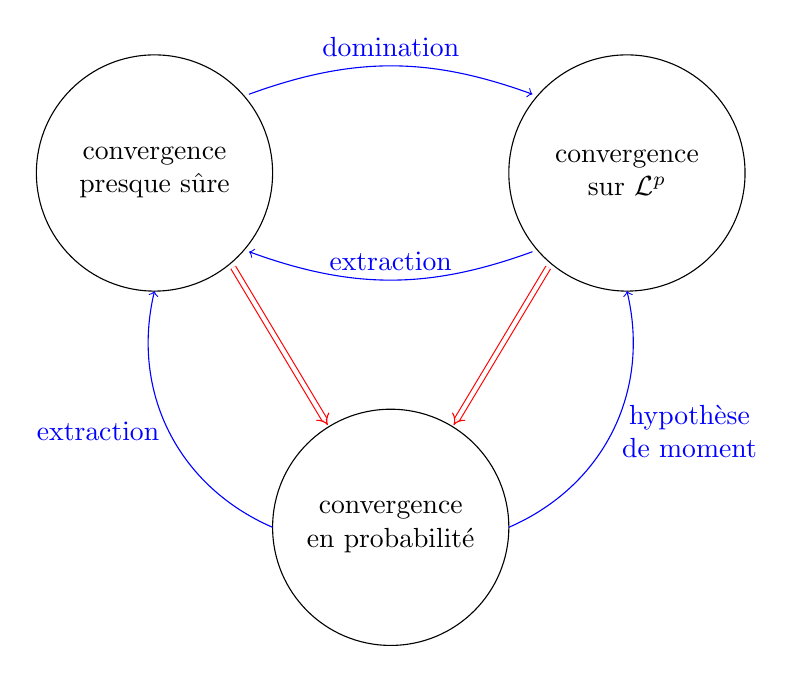
\begin{tikzpicture}[
        implies/.style={double equal sign distance, -implies},
        every node/.style={align=center}
    ]
        % Define the circle centers with labels
        \node (c1) at (-3, 2) {convergence\\presque sûre};
        \node (c2) at (3, 2) {convergence\\sur $\mathcal{L}^p$};
        \node (c3) at (0, -2.5) {convergence\\en probabilité};
        
        % Draw bigger circles around the centers
        \draw (c1) circle (1.5);
        \draw (c2) circle (1.5);
        \draw (c3) circle (1.5);
        
        % Red implication arrows (double lined) from top to bottom - now straight
        \draw[-implies, double equal sign distance, red] (-2, 0.8) -- (-0.8, -1.2);
        \draw[-implies, double equal sign distance, red] (2, 0.8) -- (0.8, -1.2);
        
        % Blue curved arrows between sets
        \draw[<-, blue] (-1.8, 1) to[bend right=20] node[above] {extraction} (1.8, 1);
        
        % Top extraction arrow now lower, mirroring the domination arrow
        \draw[<-, blue] (1.8, 3) to[bend right=20] node[above] {domination} (-1.8, 3);
        
        % Bottom arrows now start from circle sides
        \draw[->, blue] (-1.5, -2.5) to[bend left=40] node[left] {extraction} (-3, 0.5);
        
        \draw[->, blue] (1.5, -2.5) to[bend right=40] node[right] {hypothèse\\de moment} (3, 0.5);
    \end{tikzpicture}
\end{center}

\section{Loi forte des grands nombres} % 3.2

\subsection{Le résultat} % 3.2.1

\begin{theorem}[Loi forte des grands nombres]
    Soit \({(X_n)}_{n\geq 1}\) une suite de variables aléatoires
    réelles i.i.d.\ dans \(\mathcal L^1(\Omega, \scr F, \bb P)\).
    Alors
    \begin{equation*}
        \ol{X_n} = \frac{X_1 + \cdots + X_n}{n} \cvpsn \bb E[X_1].
    \end{equation*}
\end{theorem}

\begin{remark}\,
    \begin{enumerate}
        \item Si les \(X_n\) sont des variables aléatoires
        positives d'espérance infinie (\(\bb E[X_1] = +\infty\)),
        alors le théorème reste vrai au sens suivant:
        \begin{equation*}
            \frac{X_1 + \cdots + X_n}{n} \cvpsn +\infty.
        \end{equation*}

        \item La convergence est également vérifiée dans
        \(\mathcal L^1(\Omega, \scr F, \bb P)\):
        \begin{equation*}
            \frac{X_1 + \cdots + X_n}{n} \cvlpn \bb E[X_1].
        \end{equation*}
    \end{enumerate}
\end{remark}

\begin{proof}\,\\
    \ptr{} Posons \(S_n = X_1 + \cdots + X_n\) et \(S_0 = 0\).\\
    Considérons \(a\geq \bb E\ff{X_1}\)

    \ptr{} Idée: on va montrer que
    \begin{equation*}
        S_n - na \leq M < +\infty \quad\text{p.s.}
    \end{equation*}
    pour un certain \(M\). Si c'est vrai, alors
    \begin{equation*}
        \frac{S_n}{n}\leq a + \frac{M}{n} \quad\text{p.s.}
    \end{equation*}
    et donc
    \begin{equation*}
        \left(\limsup_{n\to\infty} \frac{S_n}{n}\right) \leq a \quad\text{p.s.}
    \end{equation*}
    et on conclut en faisant tendre \(a\) vers \(\bb E\ff{X_1}\).

    \ptr{} On pose
    \begin{equation*}
        M_n = \max\limits_{k=0, \ldots, n} (S_k - ka) = \max(0,X_1-a, X_1 - a + X_2 - a, \ldots, (X_1 - a) + \cdots + (X_n - a)).
    \end{equation*}
    La suite \({(M_n)}_{n\geq 0}\) est positive et croissante,
    donc elle converge presque sûrement vers
    \begin{equation*}
        M = \sup_{n\geq 0} (S_n - na)\in \ff{0, +\infty}.
    \end{equation*}

    \ptr{} \'Etape 1: montrons que \(\bb P(M=\infty) \in\{0,1\}\)\\
    Pour \(k\geq 1\), on écrit
    \begin{equation*}
        \begin{aligned}
            \{M=\infty\} 
            &= \left\{\sup_{n\geq 0} (X_1 + \cdots + X_n - na) = +\infty\right\}\\
            &= \left\{\sup_{n\geq k} (X_k + \cdots + X_n - na) = +\infty\right\}\\
        \end{aligned}
    \end{equation*}
    Ce dernier événement dépend uniquement de \(X_k, X_{k+1}, \ldots\).
    Donc il appartient à \(\ol{\scr F_k}\sigma(X_k, X_{k+1}, \ldots)\).\\
    Céci étant vrai pour tout \(k\geq 1\), on en déduit que
    \begin{equation*}
        \{M=\infty\} \in \bigcap_{k\geq 1} \ol{\scr F_k} = \scr F_\infty.
    \end{equation*}

    Les \(X_n\) étant indépendantes, la loi du 0--1 de Kolmogorov
    assure que \(\bb P(M=\infty) \in \{0,1\}\).
    
    \ptr{} \'Etape 2: montrons que \(\bb P(M=\infty) = 0\)\\
    On pose \(S_n' = X_2 + \cdots + X_{n+1}, n\geq 1\) et \(S_0' = 0\).
    Alors
    \begin{equation*}
        M'_n = \max\limits_{k=0, \ldots, n} (S_k' - ka) = \max(0, X_2 - a, X_2 - a + X_3 - a, \ldots, (X_2 - a) + \cdots + (X_{n+1} - a)).
    \end{equation*}
    On obtient la relation
    \begin{equation*}
        \begin{aligned}
            M_{n+1} 
            &= \max(0,M'_n + (X_1 - a))\\
            &= M'_n - \min(a - X_1, M'_n).
        \end{aligned}
    \end{equation*}
    Comme avant, la suite \({(M'_n)}_{n\geq 0}\) est croissante
    positive donc converge vers \(M' = \sup_{n\geq 0} (M_n' - na)\in \ff{0, +\infty}\).\\
    Comme les variables aléatoires \(X_n\) sont i.i.d., on en déduit
    que \({(S_n)}_{n\geq 0}\) et \({(S_n')}_{n\geq 0}\) ont même loi.\\
    De même, \(M_n\) et \(M_n'\) ont même loi et
    \(M\) et \(M'\) ont même loi. Alors
    \begin{equation*}
        \bb E[\min(a - X_1, M'_n)] = \underbrace{\bb E[M'_n]}_{\bb E[M_n]} - \bb E[M_{n+1}] \leq 0
    \end{equation*}
    Or, la suite \(Y_n = \min(a-X_1,M'_n)\) converge vers
    \(Y = \min(a-X_1,M')\) et vérifie \(\n{Y_n} \leq \n{a-X_1}\)
    qui est intégrable.

    On en deduit que
    \begin{equation*}
        \bb E[\min(a - X_1, M')] = \lim_{n\to\infty} \bb E[\min(a - X_1, M'_n)] \leq 0.
    \end{equation*}
    Si on suppose que \(\bb P(M=\infty) = 1\), alors
    \(\bb P(M'=\infty = 1)\) (de même loi) et donc
    \(\bb E[\min(a - X_1, M')] = \bb E[a-X_1]\), ce qui donne
    \(a\leq \bb E[X_1]\), ce qui est exclu. Donc \(\bb P(M=\infty) = 0\),
    c'est-à-dire que \(M\) est fini presque sûrement.

    \ptr{} \'Etape 3: Conclusion\\
    Comme \(M = \sup_{n\geq 0} (S_n - na)\), on obtient pour
    tout \(n\geq 0\),
    \begin{equation*}
        \begin{aligned}
            & S_n - na \leq M\\
            & \frac{S_n}{n} \leq a + \frac{M}{n}
        \end{aligned}
    \end{equation*}
    Par suite, comme \(M\) est fini p.s., on obtient
    \begin{equation*}
        \bb P\left(\left(\limsup_{n\to\infty} \frac{S_n}{n}\right) \leq a\right) = 1.
    \end{equation*}
    On en déduit que
    \begin{equation*}
        \begin{aligned}
            \bb P\left(\left(\limsup_{n\to\infty} \frac{S_n}{n}\right) \leq \bb E[X_1]\right)
            &= \bb P\left(\bigcap_{\substack{a>\bb E[X_1]\\ a\in\bb Q}}\left\{\left(\limsup_{n\to\infty} \frac{S_n}{n}\right) \leq a\right\}\right)\\
            \substack{\smol{decroissance}\\\smol{monotone}}&= \lim_{\substack{a\searrow \bb E[X_1]\\ a\in\bb Q}} \bb P\left(\left(\limsup_{n\to\infty} \frac{S_n}{n}\right) \leq a\right)\\
            &= 1.
        \end{aligned}
    \end{equation*}
    En faisant de même avec \(-X_n\), on obtient
    \begin{equation*}
        \bb P\left(\left(\liminf_{n\to\infty} \frac{S_n}{n}\right) \geq \bb E[X_1]\right) = 1.
    \end{equation*}
    Ceci prouve que
    \begin{equation*}
        \bb P\left(\limsup_{n\to\infty} \frac{S_n}{n} = \liminf_{n\to\infty} \frac{S_n}{n} = \bb E[X_1]\right) = 1.
    \end{equation*}
    donc
    \begin{equation*}
        \bb P\left(\lim_{n\to\infty} \frac{S_n}{n} = \bb E[X_1]\right) = 1.
    \end{equation*}
\end{proof}

\subsection{Applications} % 3.2.2

\subsubsection*{Marche aléatoire non centrée\label{subsubsection:marche_aleatoire_non_centree}}
\addcontentsline{toc}{subsubsection}{\nameref{subsubsection:marche_aleatoire_non_centree}}
\setcounter{subsubsection}{1}

Soit \({(X_n)}_{n\geq 1}\) une suite de variables aléatoires
réelle i.i.d.\ intégrables. On pose \(S_n = X_1 + \cdots + X_n\).
On appelle souvent \({(S_n)}_{n\geq 1}\) une \defemph{marche aléatoire}.

\begin{example}
    On considère \({(X_n)}_{n\geq 1}\) une suite de variables aléatoires
    réelles i.i.d.\ comme suit:
    \begin{equation*}
        X_n=\begin{cases}
            1 & \text{avec probabilité } p\\
            -1 & \text{avec probabilité } 1-p
        \end{cases}
    \end{equation*}

    \begin{center}
    \begin{tikzpicture}
        \begin{axis}[
            xlabel = \(n\),
            xmin = 0,
            xmax = 10,
            ymin = -1, % Ensures some space below the x-axis
            ymax = 3,
            width = 12cm, % Makes x-axis longer
            height = 5cm, % Adjusts graph height
            axis lines = middle, % Places x-axis at y=0 and y-axis at x=0
            xtick = {0,1,2,3,4,5,6,7,8,9,10}, % Ensures all x values are shown
            ytick = {-1,0,1,2,3}, % Custom y-ticks
            every axis x label/.style={at={(ticklabel* cs:1.05)},anchor=north}, % Moves x-label below axis
            every axis y label/.style={at={(ticklabel* cs:1.05)},anchor=east}, % Moves y-label left of axis
        ]
            % Add points in order and link them with a broken line
            \addplot [
                color=red,
                mark=*,
            ]
            coordinates {
                (0,0)
                (1,1)
                (2,2)
                (3,1)
                (4,2)
                (5,3)
                (6,2)
                (7,1)
                (8,2)
                (9,1)
            };
            \node[red] at (axis cs:9,1) {\(\bullet\)};
            \node[anchor=west, red] at (axis cs:9,1) {\(S_9\)};
        \end{axis}
    \end{tikzpicture}
\end{center}

    Dans le cas général, supposons que \(\bb E[X_1] \neq 0\).
    La loi forte des grands nombres donne alors
    \begin{equation*}
        \frac{S_n}{n} \cvpsn \bb E[X_1] 
    \end{equation*}
    donc
    \begin{equation*}
        \n{\frac{S_n}{n}} \cvpsn +\infty,\qquad \left(\bb P\left(\n{S_n} \cvn +\infty\right) = 1\right). 
    \end{equation*}

    \subsubsection*{Approximation d'intégrales}\label{subsubsection:approximation_d_integrales}
    \addcontentsline{toc}{subsubsection}{\nameref{subsubsection:approximation_d_integrales}}
    \setcounter{subsubsection}{2}

    Soit \(f:\bb R\to\bb R\) une fonction intégrable. On
    souhaite calculer
    \begin{equation*}
        \int_0^1 f(x) \der\lambda_1(x).
    \end{equation*}
    Souvent, on ne sait pas faire donc on cherche une valeur
    approchée. Soient \(U_1,\ldots,U_n\) des variables
    aléatoires indépendantes de loi uniforme sur \([0,1]\).
    Alors, les variables aléatoires \(f(U_1),\ldots,f(U_n)\)
    sont i.i.d.\ et intégrables donc la loi forte des grands
    nombres donne
    \begin{equation*}
        \frac{f(U_1) + \cdots + f(U_n)}{n} \cvpsn \bb E[f(U_1)] = \int_0^1 f(x) \der\lambda_1(x).
    \end{equation*}

    \ptr{} Avantages de la méthode: aucune hypothèse
    de régularité sur \(f\) et extensible au cas
    \(f:\bb R^d\to\bb R\) (en considérant 
    \(U_1,\ldots,U_n\) uniformes sur \([0,1]^d\)).

    \ptr{} Inconvénient: convergence lente (en \(\sqrt n\)).

    Cette méthode est appelée \defemph{méthode de Monte-Carlo}.
\end{example}